% PP-Article.tex for AEA last revised 22 June 2011
\documentclass[twocolumn, a4paper]{article}

%%%%%% NOTE FROM OVERLEAF: The mathtime package is no longer publicly available nor distributed. We recommend using a different font package e.g. mathptmx if you'd like to use a Times font.
\usepackage{mathptmx}
\usepackage{amsmath}
\usepackage[dutch]{babel}
\usepackage{subcaption}
\usepackage[width=.8\textwidth]{caption}
\usepackage{float}
\usepackage{hyperref}
\usepackage[utf8]{inputenc}
\usepackage{booktabs}
\usepackage{multicol}
\usepackage{longtable}
\usepackage{minted}
% If you have trouble with the mathtime package please see our technical support 
% document at: http://www.aeaweb.org/templates/technical_support.pdf
% You may remove the mathtime package if you can't get it working but your page
% count may be inaccurate as a result.
% \usepackage[cmbold]{mathtime}
\usepackage{xargs}                      % Use more than one optional parameter in a new commands 
\usepackage[pdftex,dvipsnames]{xcolor}  % Coloured text etc.
% 
\usepackage{pdfpages}
\usepackage[colorinlistoftodos,prependcaption,textsize=tiny]{todonotes}
\newcommandx{\unsure}[2][1=]{\todo[linecolor=red,backgroundcolor=red!25,bordercolor=red,#1]{#2}}
\setlength{\marginparwidth}{2cm}
% Note: you may use either harvard or natbib (but not both) to provide a wider
% variety of citation commands than latex supports natively. See below.

% Uncomment the next line to use the natbib package with bibtex 
%\usepackage{natbib}
\usepackage{titlesec}

\titlespacing*\section{0pt}{12pt plus 4pt minus 2pt}{0pt plus 2pt minus 2pt}
\titlespacing*\subsection{0pt}{12pt plus 4pt minus 2pt}{0pt plus 2pt minus 2pt}
\titlespacing*\subsubsection{0pt}{12pt plus 4pt minus 2pt}{0pt plus 2pt minus 2pt}



% Uncomment the next line to use the harvard package with bibtex
%\usepackage[abbr]{harvard}

% This command determines the leading (vertical space between lines) in draft mode
% with 1.5 corresponding to "double" spacing.
\begin{document}

\title{Geavanceerde computerarchitectuur: Labo 02' \\ 
\large{Uitbreiding: OpenCL} \\
\small{\url{https://github.com/iPieter/JLIZNN_CUDA_and_openCL}}}
\author{\textsc{Anton Danneels en Pieter Delobelle}}
\date{}
\maketitle

\section{Inleiding}
Dit verslag is geschreven als extra opdracht voor het labo geavanceerde computerarchitectuur. Het OpenCL framework wordt toegelicht en getest op dezelfde scenario's als bij het labo over CUDA. Daarnaast is er een \emph{pipeline} opgezet om afbeeldingen te bewerken en meerdere filters toe te passen in één operatie. Dit is dan als \emph{cross platform} applicatie gebundeld. 

\section{Analyse}

\subsection{OpenCL}
OpenCL is---net als CUDA---een framework en platform om berekeningen te kunnen uitvoeren op GPU's, maar biedt ook meer flexibiliteit door ook CPU's en andere \emph{hardware accelerators} te ondersteunen. Daarnaast is OpenCL ook een open standaard die door verschillende fabrikanten wordt gevolgd, in tegenstelling tot CUDA van NVIDEA.

Omdat OpenCL meerdere \emph{vendors} en systemen ondersteunt, is er een hiërarchische organisatie om verschillende apparaten aan te sturen. Ten eerste zijn gelijkaardige systemen gegroepeerd per \emph{platform}. OpenCL-kernels worden gecompileerd voor een bepaald platform. 

Ten tweede worden platformen opgedeeld in \emph{devices}. Dit is iedere CPU, GPU of andere \emph{hardware accelerator} onder een bepaald platform. Logischerwijs heeft ieder apparaat enkele eigenschappen, zoals kloksnelheid en het aantal \emph{work units}, die een invloed hebben op de resulterende uitvoersnelheid voor een bepaalde kernel.

\begin{minted}{c}
    const int2 pos = {
            get_global_id(0), 
            get_global_id(1)
        };
    \end{minted}
    \label{c:index}

Iedere OpenCL-kernel wordt uitgevoerd door één of meerdere \emph{work items}, wat equivalent is aan een CUDA-thread. Alle items krijgen enkele indices toegewezen: een globale index, een index binnen de work unit (local id) en de index van de work unit. Deze items worden dus gegroepeerd in blokken, die conceptueel overeenkomen met de \emph{wraps} uit CUDA. 

Omdat OpenCL echter ook op CPU's draait, is het kiezen van een optimale \emph{local work size} echter complexer. Hiervoor biedt OpenCL de optie om dit op NULL te laten, waardoor automatisch de beste grootte gekozen wordt.

\subsection{Kleurenruimte en kleurendiepte}
Verschillende operaties werken intern met een kleurendiepte die groter is dan de standaard diepte waarin een afbeelding wordt ingelezen (8 bits per component). Dit is problematisch voor operaties zoals vervagen, aangezien convoluties hier voor resultaten kunnen zorgen die groter zijn wat kan weergegeven worden in een getal van 8 bits (256). Een optie is hiervoor om grotere representaties te gebruiken, maar dit stelt het probleem enkel uit. Hierom is gekozen om intern te werken met een zwevendekommagetal (\emph{double}) Pas finaal worden alle waarden gecast naar een 8-bits getal.

Een tweede kwestie is in welke kleurruimte operaties uitgevoerd worden. Standaard worden bestanden ingelezen in RGB of RGBA indien er een \emph{alpha}-kanaal aanwezig is, maar andere kleurruimtes kunnen voor bepaalde operaties voordeliger zijn.

\begin{itemize}
    \item \textbf{RGB}: populair systeem dat kleuren encodeerd in 3 componenten, rood, groen en blauw. In het geval van RGB24 zijn er 16 miljoen kleuren mogelijk, maar voor recente ontwikkelingen omtrent \emph{high dynamic range} (HDR) is dit niet altijd meer toereikend. De meeste afbeeldingen zijn hierin echter zonder problemen te encoderen. 

    Bepaalde bewerkingen, zoals het aanpassen van saturatie, zijn echter zeer complex in RGB. 

    Daarnaast is het ook mogelijk om de RBG-ruimte niet-lineair te encoderen. Hierdoor kunnen bijvoorbeeld meer discrete zwartwaarden onderscheiden worden. Hiervoor wordt een parameter $\gamma$ geïntroduceerd.
    
    \item \textbf{HSL}: dit systeem encodeert de tint (\emph{hue}), saturatie en helderheid (\emph{lightness}) van een pixel. Het spreekt voor zich dat het aanpassen van deze componenten hierin zeer eenvoudig is. De tint kan voorgesteld worden in een kleurenwiel, wat dit systeem ook geschikt maakt voor kleureninput van gebruikers. Kleuren kunnen echter wel afwijken door interpolaties, wat het minder geschikt maakt voor bepaalde applicaties.

    \item \textbf{HSI}: Variant op HSL, maar met een intensiteit-parameter in plaats van de helderheid.  
    \item \textbf{CMYK}: additief kleurensysteem voor drukwerk, voor digitale verwerking biedt dit geen voordelen. 
    \item \textbf{CIE XYZ}: systeem gebaseerd op perceptie. Er is één helderheidscomponent (Y) en twee kleurencomponenten (X en Z). Dit systeem is zeer bruikbaar voor het mixen van kleuren.
    \item \textbf{CIElab}: Een tweede systeem met twee kleurencomponenten en een helderheidscomponent. Hier worden kleuren geëncodeerd als \emph{Luminance} en een combinatie van rood-groen en blauw-geel. Het is minder bruikbaar voor kleurtransformaties, maar is uniform (in tegenstelling to gequantiseerde modellen zoals RGB). Dit systeem wordt in Photoshop gebruikt als intermediaire representatie bij het converteren tussen kleurensystemen.
\end{itemize}

Voor de meeste operaties is een RBG-ruimte dus prima te doen, waarbij eventueel kan overgeschakeld worden naar CIE XYZ als intermediaire voorstelling mocht het mixen van kleuren gewenst zijn. Voor de invoer van kleuren door de gebruiker zijn twee opties mogelijk, afhankelijk van het gewenste doel. HSL is intuïtief voor de gebruiker, zeker in combinatie met een \emph{color picker}. Voor operaties zoals witpuntsbepaling is dit echter een omweg en kan beter direct voor RGB gekozen worden. 

\subsection{Gaussiaans vervagen}
Om OpenCL uit te testen werd een \textit{mask} toegepast op een afbeelding. Dit mask combineert pixels rondom een gekozen doelpixel, waarbij elke pixel een bepaald gewicht krijgt. E\'en van deze masks is de Gaussiaanse. Hierbij krijgen de pixels een gewicht gebaseerd op hun afstand tot het doelwit. De gewichten volgen zo een Gaussiaanse functie.

Om de masks niet te moeten \emph{hardcoden}, kunnen deze iteratief gegenereerd worden op basis van een rij uit het binomium van Newton. Dit maakt dus gebruik van geheeltallige waarden, niet van reële getallen zoals een echte Gaussiaanse verdeling. Hierdoor verdonkeren afbeeldingen echter niet, aangezien er geen afrondingsfouten optreden. 

\begin{equation*}
    \begin{pmatrix}
        1 \\
        4 \\
        6 \\
        4 \\
        1
    \end{pmatrix}
    \cdot
    \begin{pmatrix}
        1 & 4 & 6 & 4 & 1
    \end{pmatrix}
    =
    \begin{pmatrix}
        1 & 4 & 6 & 4 & 1 \\
        4 & 16 & 24 & 16 & 4 \\
        6 & 24 & 36 & 24 & 6 \\
        4 & 16 & 24 & 16 & 4 \\
        1 & 4 & 6 & 4 & 1
    \end{pmatrix}
\end{equation*}

Het verband tussen het binomium van Newton en de resulterende mask is hierboven weergegeven. Op basis van deze eigenschap is het dus ook mogelijk om de operatie significant te versnellen door de convolutie in twee passen te doen over een afbeelding, met de binominale reeks in plaats van het resulterende masker. 

\subsection{Witpuntsverschuiving}
Het verschuiven van een witpunt van een afbeelding is een vorm van kleurencorrectie, waarbij het witpunt verschoven kan worden in een kleurenruimte. Indien een kleur in het RGB24-profiel geselecteerd is als witpunt, is de volgende transformatie mogelijk:

%schaamteloos :fancy-pirate: van wikipedia
\begin{equation}
\left[\begin{array}{c} R \\ G \\ B \end{array}\right]=\left[\begin{array}{ccc}\frac{255}{R'_w} & 0 & 0 \\ 0 & \frac{255}{G'_w} & 0 \\ 0 & 0 & \frac{255}{B'_w}\end{array}\right]\left[\begin{array}{c}R' \\ G' \\ B' \end{array}\right]
\end{equation}

\subsection{Qt}
Qt is een \emph{cross-platform} raamwerk voor gebruikersinterfaces te ontwikkelen, waarbij de achterliggende code in C++ geschreven kan worden. Het raamwerk volgt een object-geörienteerde strategie, door iedere GUI-element te modelleren als een object (QWidget) met hiërarchische overerving voor verschillende types van elementen, zoals knoppen (QButton).

\begin{figure*}[htb]
    \centering
    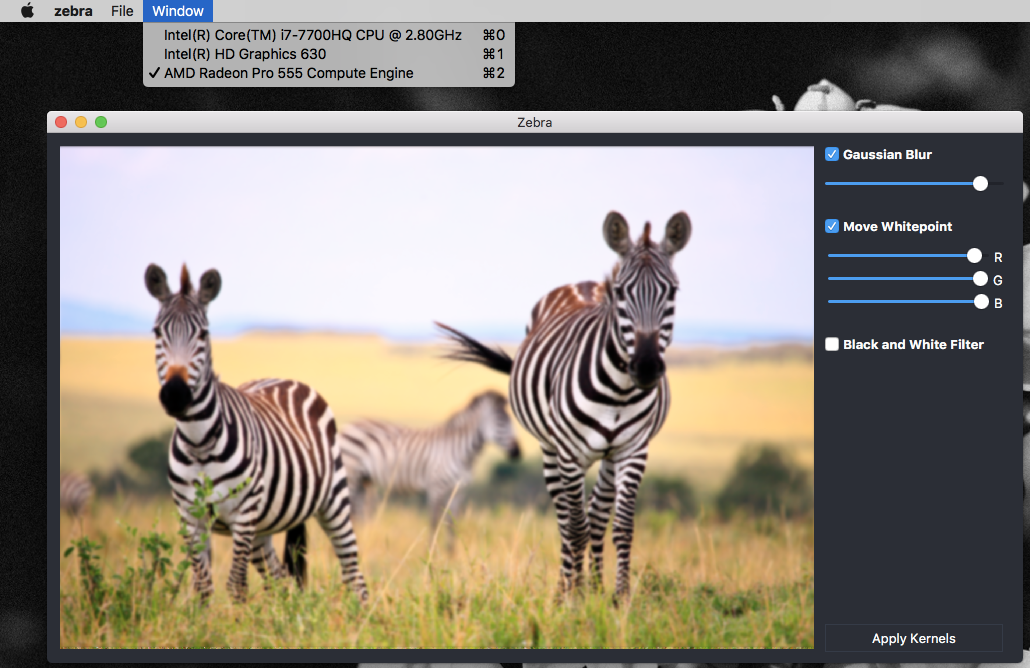
\includegraphics[width=0.8\textwidth]{screenshot.png}
    \caption{Screenshot van de applicatie.}\label{fig:gui}
\end{figure*}
\newpage

\section{Oplossing}

\subsection{Pipeline}
Voor een foto verwerkt kan worden door een kernel moet eerst de OpenCL omgeving geconfigureerd worden. Dit bestaat uit de volgende stappen:

\begin{enumerate}
    \item Platforms en devices opvragen 
    \item Context aanmaken
    \item Programma compileren
    \item Command queue aanmaken
    \item Kernels configureren
\end{enumerate}
Pas indien dit gebeurd is, kan kernel op de command queue gezet worden zodat deze uitgevoerd kan worden. Om de resultaten uit te lezen wordt er gewacht op de command queue en vervolgens kan een leesopdracht gegeven worden aan de command queue. 

Om grotere hoeveelheden data naar de kernels te uploaden, wordt gebruik gemaakt van buffer objecten. Deze specificeren hoe de data er uit ziet en hoe groot deze is. In deze applicatie worden buffers gebruikt om de afbeeldingen en een kopie van de afbeelding door te sturen naar de kernel, samen met een mask.

\subsection{Apparaatselectie}
Eerder is geïntroduceerd dat OpenCL met meerdere \emph{devices} over meerdere platformen kan werken. Voor bewerkingen op afbeeldingen lijkt het evident om een parallel apparaat te kiezen, wat OpenCL automatisch kan doen door middel van een \emph{flag}. 

Aangezien dit systeem echter dient om beide te vergelijken, is er gekozen om alle apparaten op te vragen via de OpenCL-API en ter beschikking te stellen in de GUI. De gebruiker kan dan zelf kiezen op welk apparaat de pipeline uitgevoerd wordt, waarbij het zelfs dezelfde pipeline op meerdere devices kan uitvoeren. 

\subsection{GUI}
De GUI is geschreven in Qt, waarbij gekozen wordt voor een venster met primaire focus op de geopende foto en de besturingselementen aan de rechterkant. Een schermafbeelding van de applicatie---die Zebra gedoopt is---is te zien in Figuur~\ref{fig:gui} 

\begin{figure}
    \centering
    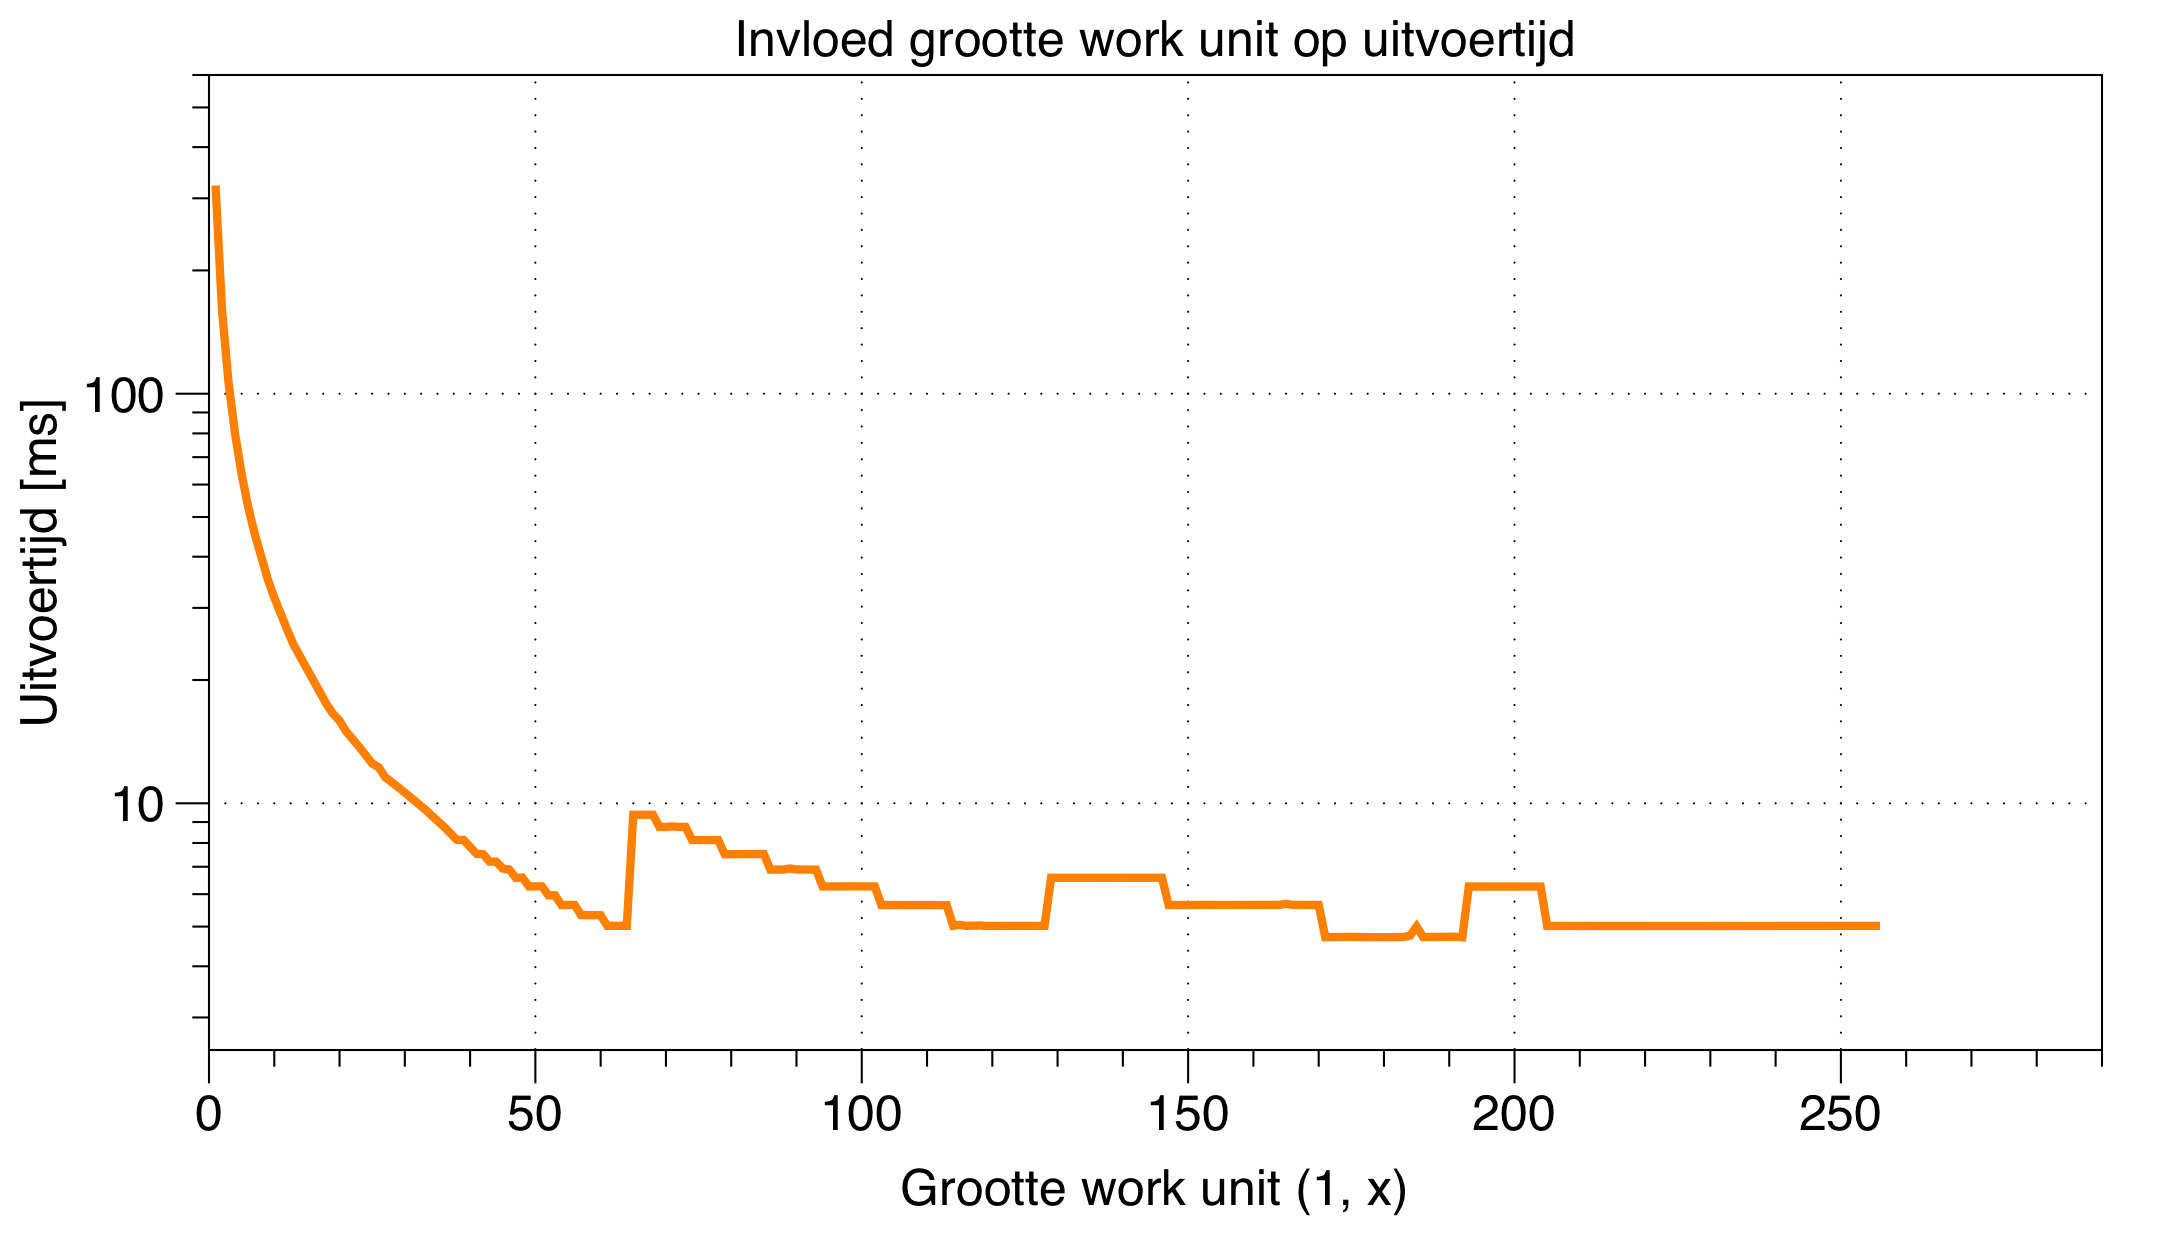
\includegraphics[width=0.48\textwidth]{data/execution-time.png}
    \caption{Invloed van \emph{work size} op uitvoertijd.}\label{fig:output-one}
\end{figure}

\begin{figure}
    \centering
    \begin{subfigure}{0.48\textwidth}
        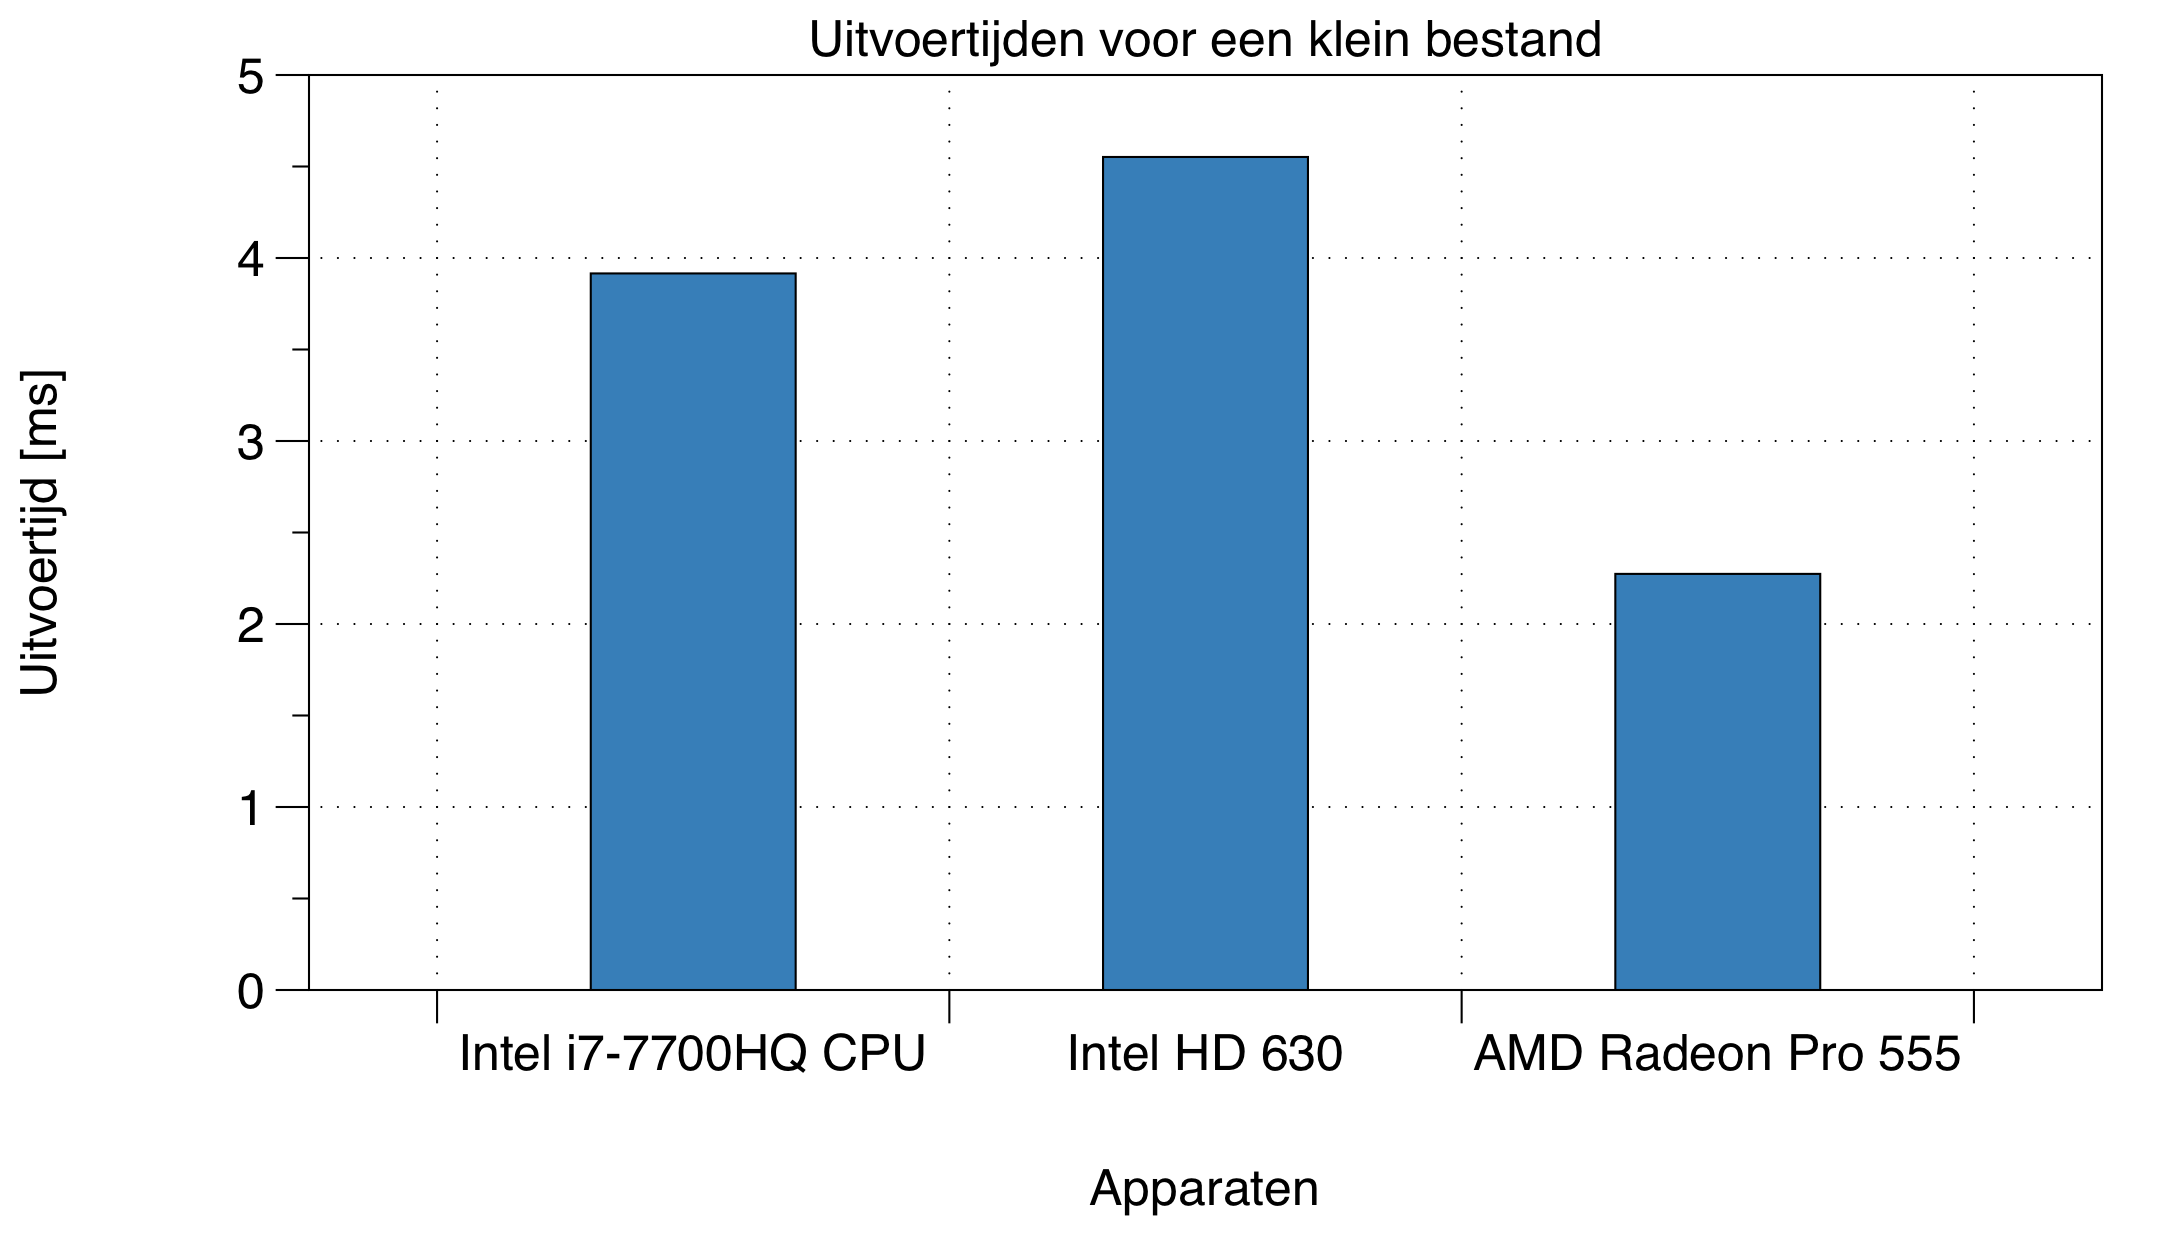
\includegraphics[width=\textwidth]{data/klein.png}
    \end{subfigure}
    \begin{subfigure}{0.48\textwidth}
        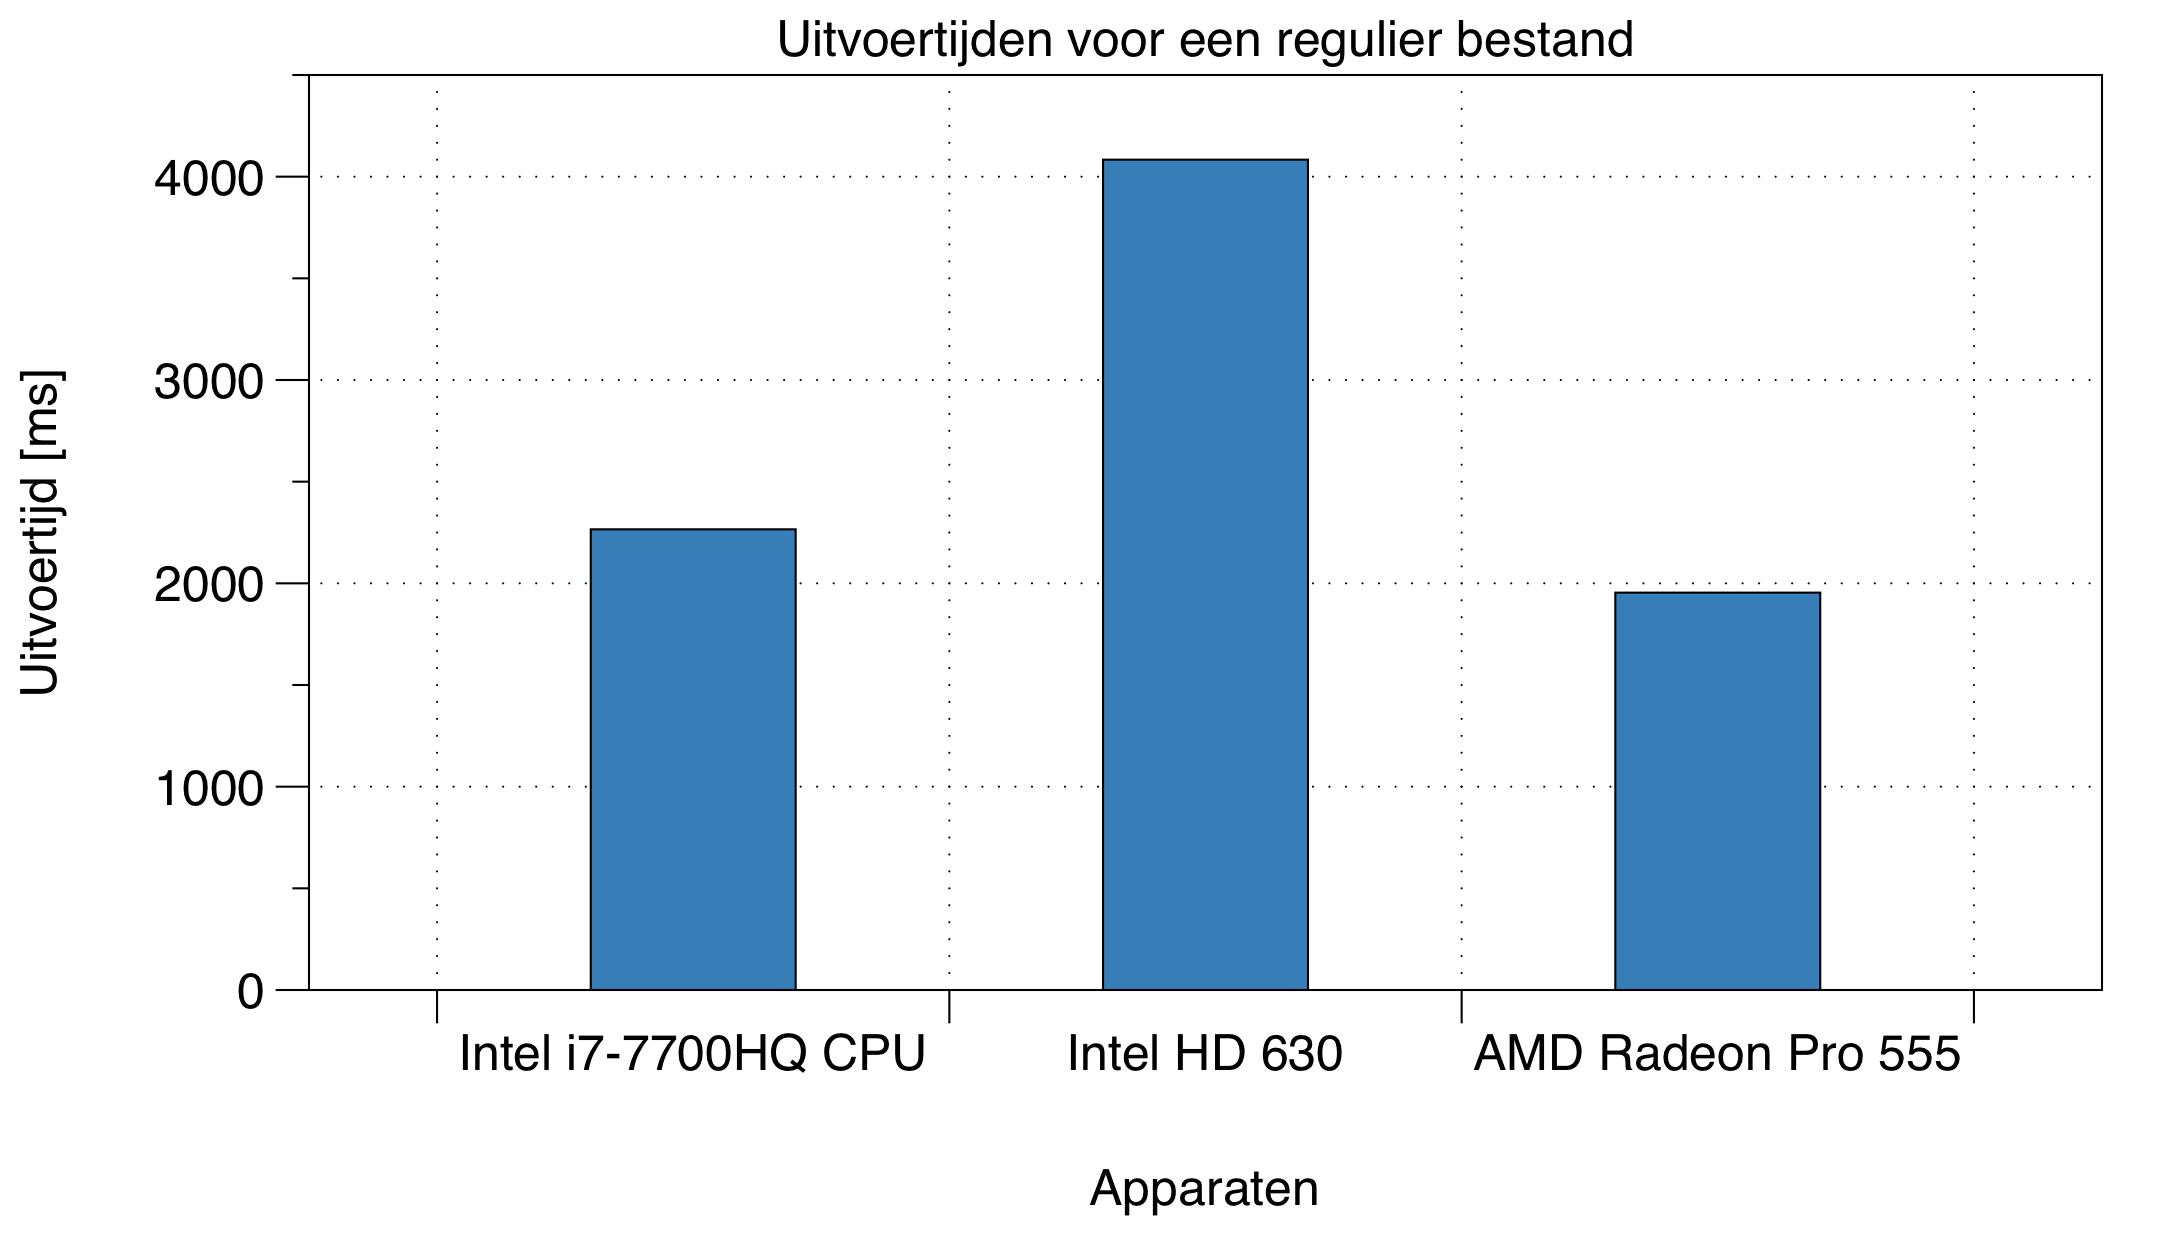
\includegraphics[width=\textwidth]{data/normaal.png}
    \end{subfigure}
    \begin{subfigure}{0.48\textwidth}
        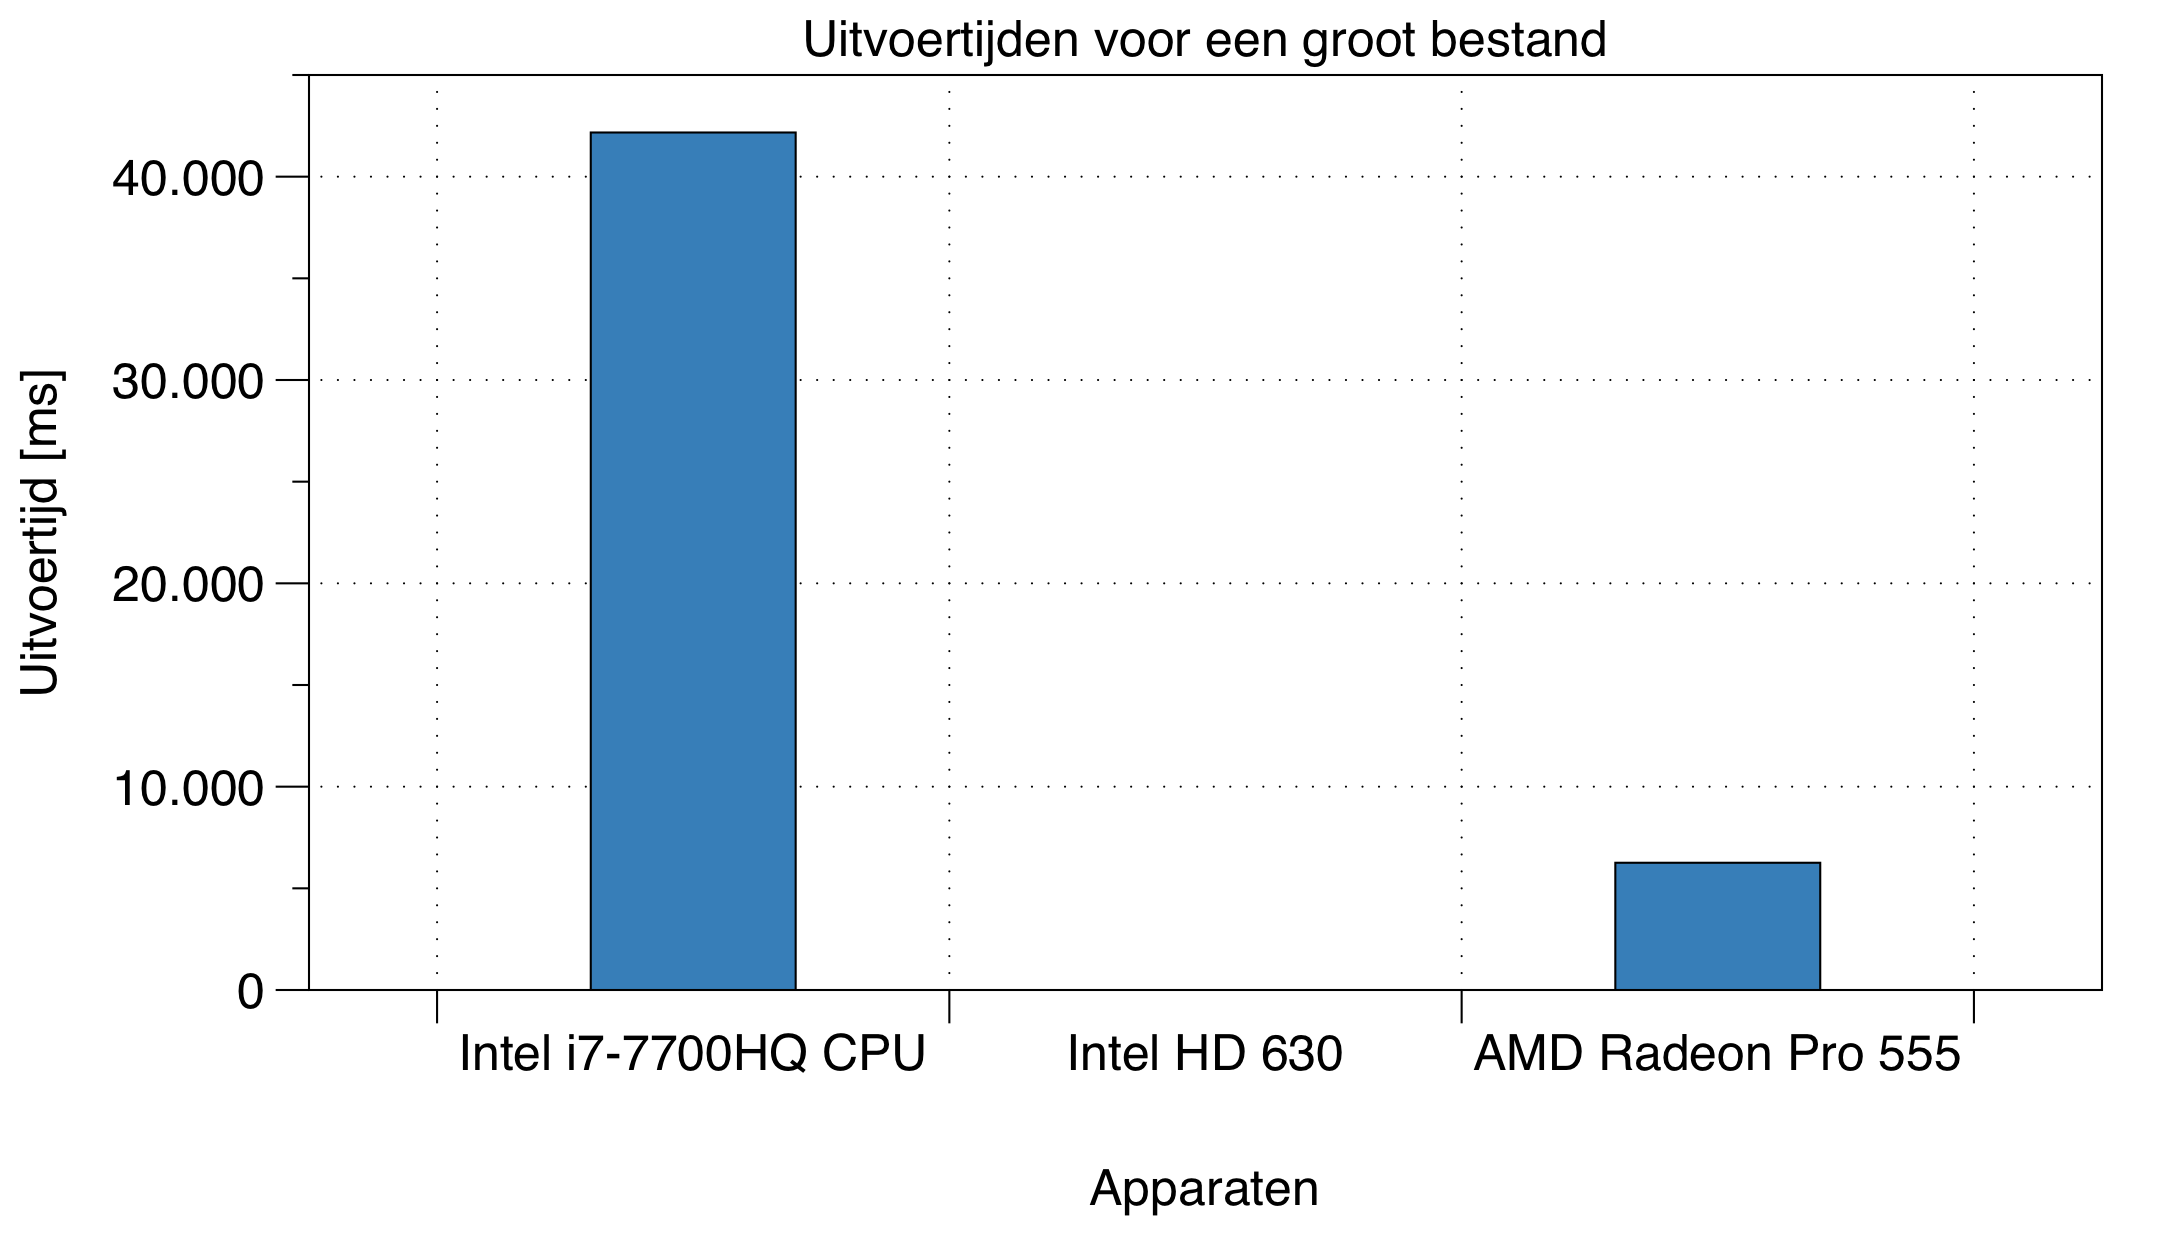
\includegraphics[width=\textwidth]{data/groot.png}
    \end{subfigure}
    \caption{Grafische voorstelling van de data uit Tabel~\ref{table:measurements}.}\label{fig:images}
\end{figure}

\newpage

\section{Evaluatie}

\subsection{Invloed van local work size}
Zoals eerder vermeld, hebben verschillende devices een verschillende hardwareconfiguratie. Hierdoor zijn bepaalde dimensies langzamer---aangezien de hardware niet ideaal gebruikt wordt---of zelfs niet mogelijk. Ieder device kan zijn eigen maxima rapporteren, wat voor een CPU veelal één is.

Voor een GPU (AMD Radeon Pro 555 Compute Engine) is een meting uitgevoerd over alle combinaties van 1x1 tot 128x128. Hiervoor is een afbeelding van 1024x1024 van een zebra gekozen, met vier kleurencomponenten (RGBA). Per dimensie zijn er 5 metingen uitgevoerd. Hier resultaat is grafisch te zien in Figuur~\ref{fig:output-all}. De data staat ook op Github. Een tweede meting is uitgevoerd voor een grotere \emph{work size}, maar volgens 1 dimensie. Het resultaat daarvan is te zien in Figuur~\ref{fig:output-one}.



Op basis van deze data zijn enkele observaties te maken. Zo is een kleine \emph{work size} zeer nadelig voor de uitvoeringssnelheid. Dit is in het bijzonder terug te zien voor een grootte van 1x1. Aangezien hierdoor maar 1 thread per \emph{work unit} gebruikt wordt, is het vanzelfsprekend dat dit een slechter resultaat oplevert.

Een tweede observatie is dat de uitvoeringstijd boven $work size_x > 64$ terug wat toeneemt. Dit is vermoedelijk gedeeltelijk te wijten aan het feit dat de gebruikte afbeelding wordt opgedeeld in blokken, waardoor er een blok benodigd is dat niet volledig gevuld kon worden. Daarnaast is een compute unit van AMD ook 64 work units groot, wat verklaart waarom op veelvouden van 64 de beste performantie te zien is. Dit is duidelijk te zien in Figuur~\ref{fig:output-one}

\begin{table*}[]
    \centering
    \caption{Vergelijking tussen die OpenCL-devices op eenzelfde systeem, waarbij 5 keer een Gaussiaanse vervaging is toegepast.}\label{tab:mes}
    \label{table:measurements}
    \begin{tabular}{@{}llrrr@{}}
        \toprule
        Abeelding & Formaat (w, h, comp) & Intel i7-7700HQ CPU {(}ms{)} & Intel HD 630 {(}ms{)} & AMD Radeon Pro 555 {(}ms{)} \\ \midrule
        bob.jpg   & 48 x 64 x 3              & 3.9157                       & 4.552                 & 2.2738                      \\
        zebra.jpg & 2048 x 1365 x 3      & 2265.7                       & 4083.6                & 1954.3                      \\
        paris.jpg & 11661 x 3581 x 4 & 42172 &Kernel beïndigt& 6257.6 \\ \bottomrule
    \end{tabular}
\end{table*}

\subsection{Vergelijking tussen devices}
Aangezien OpenCL voor meerdere \emph{devices} en types van apparaten werkt, is het gemakkelijk deze te vergelijken. Daarnaast ondersteunt de GUI deze selectie ook, waardoor meerdere ingebouwde devices eenvoudig te benchmarken zijn. In dit geval zijn drie foto's vijf keer vervaagd op de drie OpenCL-devices in een Macbook Pro 2018 15". Hier resultaat hiervan is weergeven in Tabel~\ref{tab:mes} en grafisch in Figuur~\ref{fig:images}.

Hierbij valt op te merken dat het initialiseren van een kernel niet in de metingen ingenomen zit, aangezien deze kernels persistent kunnen blijven op het apparaat. Een van de voordelen is tenslotte dat er een pipeline gemaakt kan worden, die op \emph{streaming data} inwerkt. 

Op basis van de metingen vallen er een aantal observaties te maken. Ten eerste presteert de ingebouwde GPU van Intel ondermaats en weigert deze zelfs de grootste afbeelding te verwerken. Dit is vermoedelijk te wijten aan de opbouw van de pipeline, waardoor deze lang in één kernel kan blijven zitten. Dit blijkt geen probleem te zijn voor de andere twee apparaten, maar voor de Intel GPU wel. Ook zijn sommige afbeeldingen hierdoor niet volledig correct verwerkt. Aangezien de kernel correct functioneert op twee andere apparaten, is hier niet verder op ingegaan.

Daarnaast valt er op te merken dat de prestaties van de dedicated GPU stukken beter zijn voor het zeer kleine bestand én het zeer grote bestand. Maar niet voor een bestand van 2048 x 1365 pixels. Voor het grote bestand is een snelheidswinst te verwachten, en bij kleinere bestanden is het dan ook weer logisch dat de snelheidswinst minder wordt door de kost van het initialiseren ten opzichte van de CPU. Dit verwachtingspatroon is ook terug te zien in de normale en grote afbeeldingen. 

De kleine afbeelding wijkt echter af van dit patroon. Aangezien het een zéér kleine afbeelding betreft (750 bytes), kunnen andere factoren een rol spelen. Zo moet OpenCL ook voor op de CPU een proces met meerdere threads aanmaken, wat mogelijks nog kostelijker is dan dit op de GPU te doen. 

\subsection{Vergelijking met CUDA}
Figuur~\ref{fig:vs} geeft de \emph{speedup factor} weer van beide systemen ten opzichte van een \emph{single-theaded} equivalente operatie op de CPU. Hiervoor is de code van een eerder labo gebruikt, wat op een systeem met een GeForce GT 750M uitgevoerd is. 

Daarnaast is in Figuur~\ref{fig:vs-overhead} ook de overhead weergegeven voor een afbeelding. Hierbij is voor OpenCL de setup (kernel initialiseren, command queue opzetten) apart gemeten, aangezien dit een eenmalige operatie is. 

Uit deze metingen valt een enigszins onverwachte conclusie te trekken: OpenCL is ongeveer 20x langzamer is over alle metingen. Mogelijks is dit te wijten aan het feit dat (oudere) NVIDEA GPU's slechtere ondersteuning hebben voor OpenCL.

\begin{figure}
    \centering
    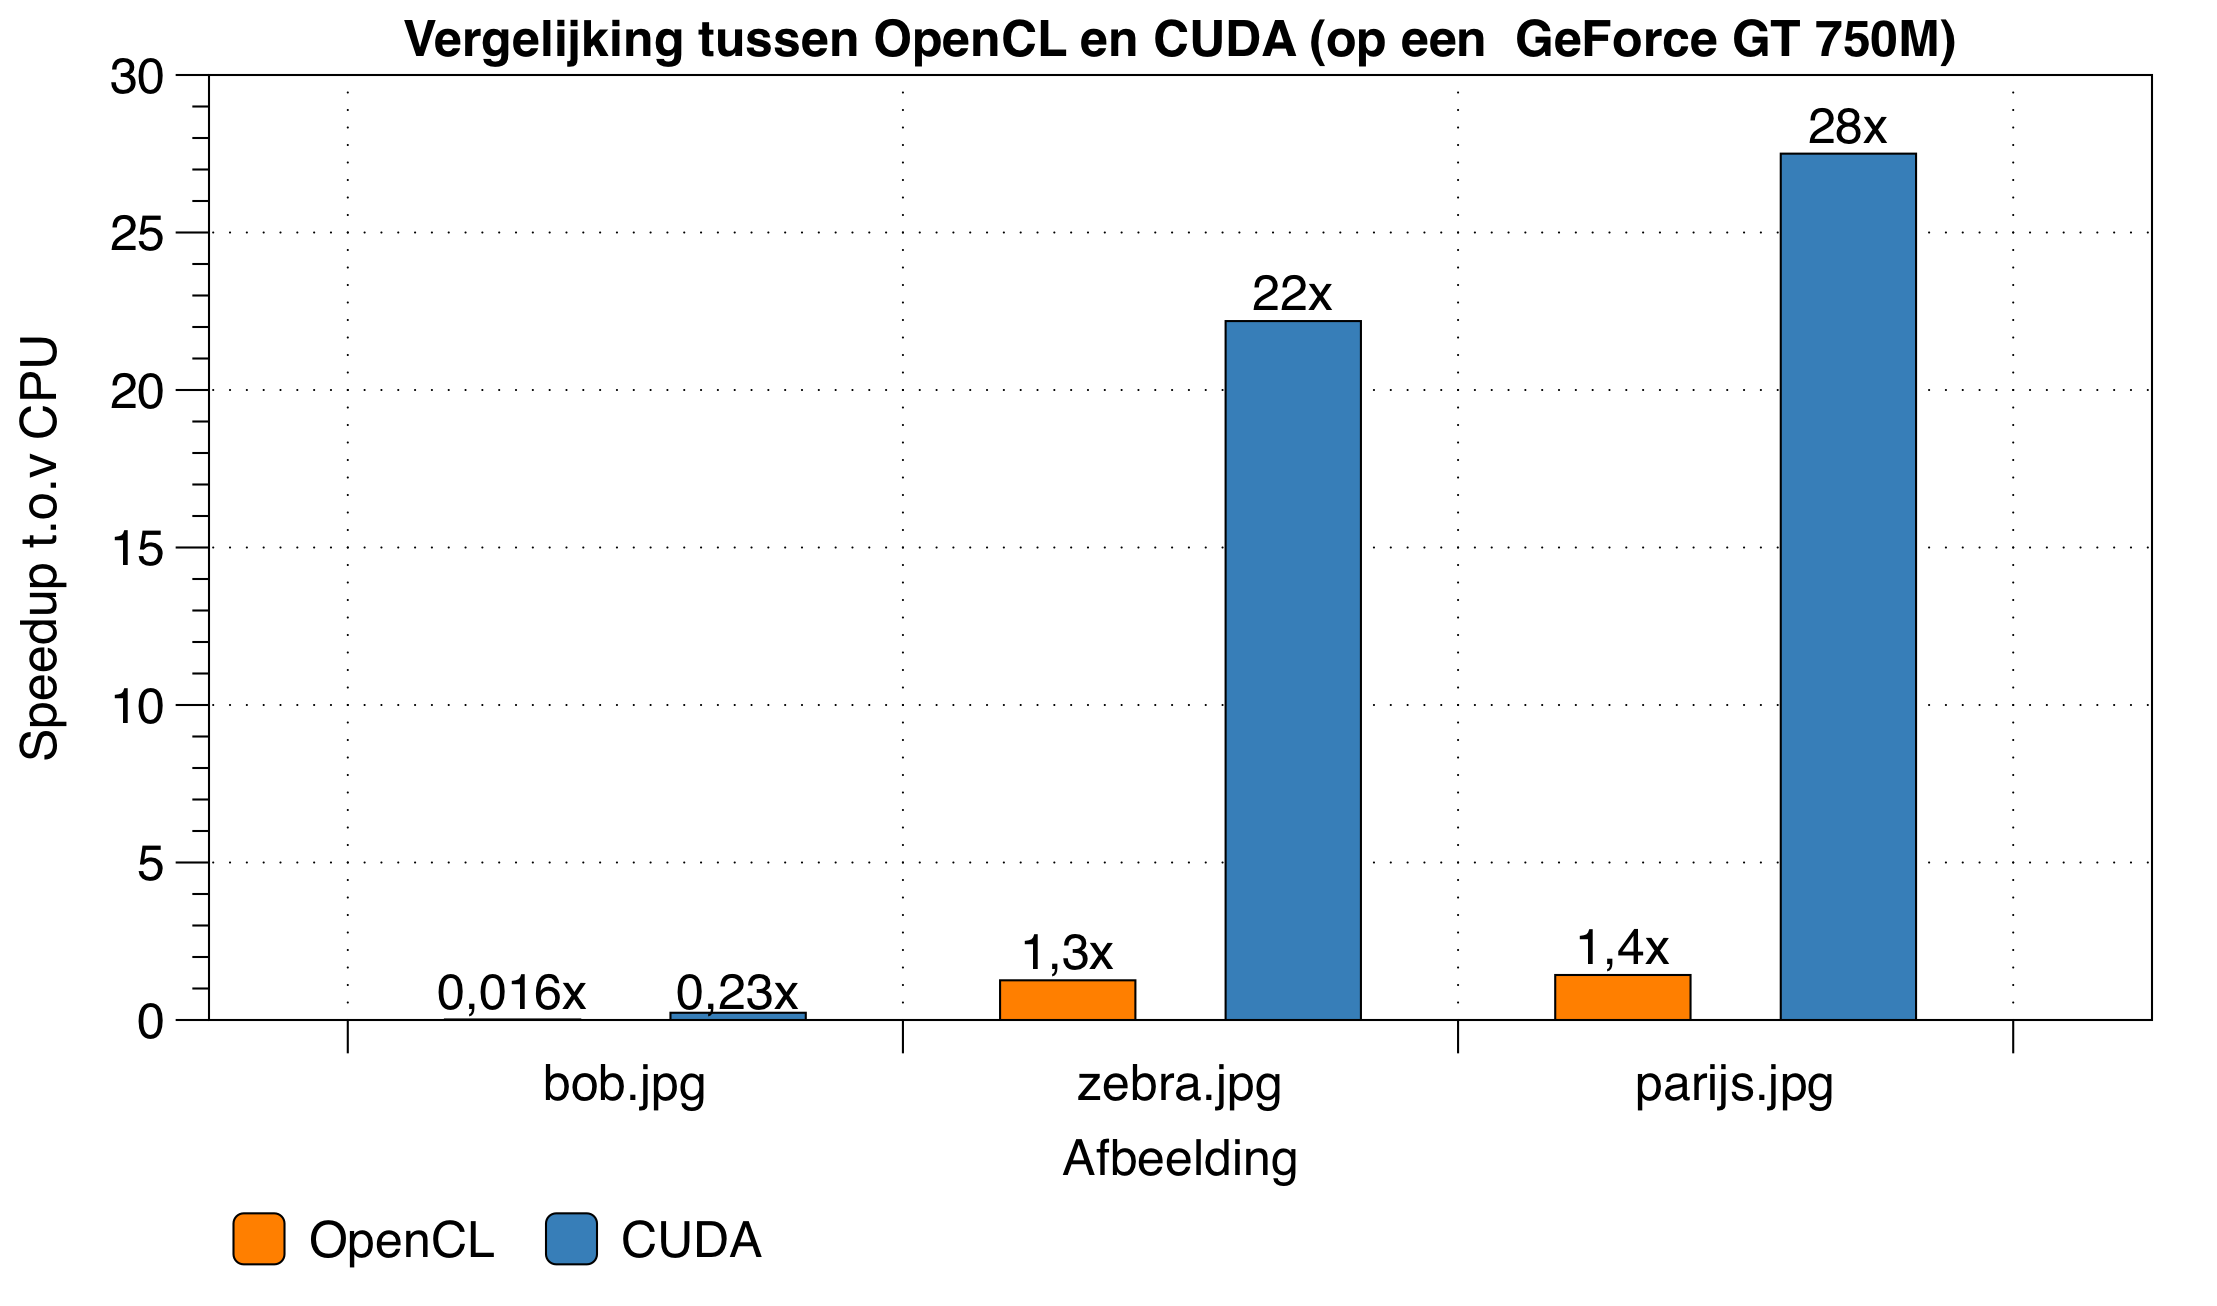
\includegraphics[width=0.48\textwidth]{data/opencl-vs-cuda.png}
    \caption{Speedup van Gaussiaans vervagen \\in OpenCL en CUDA t.o.v. de CPU.}\label{fig:vs}
\end{figure}

\begin{figure}
    \centering
    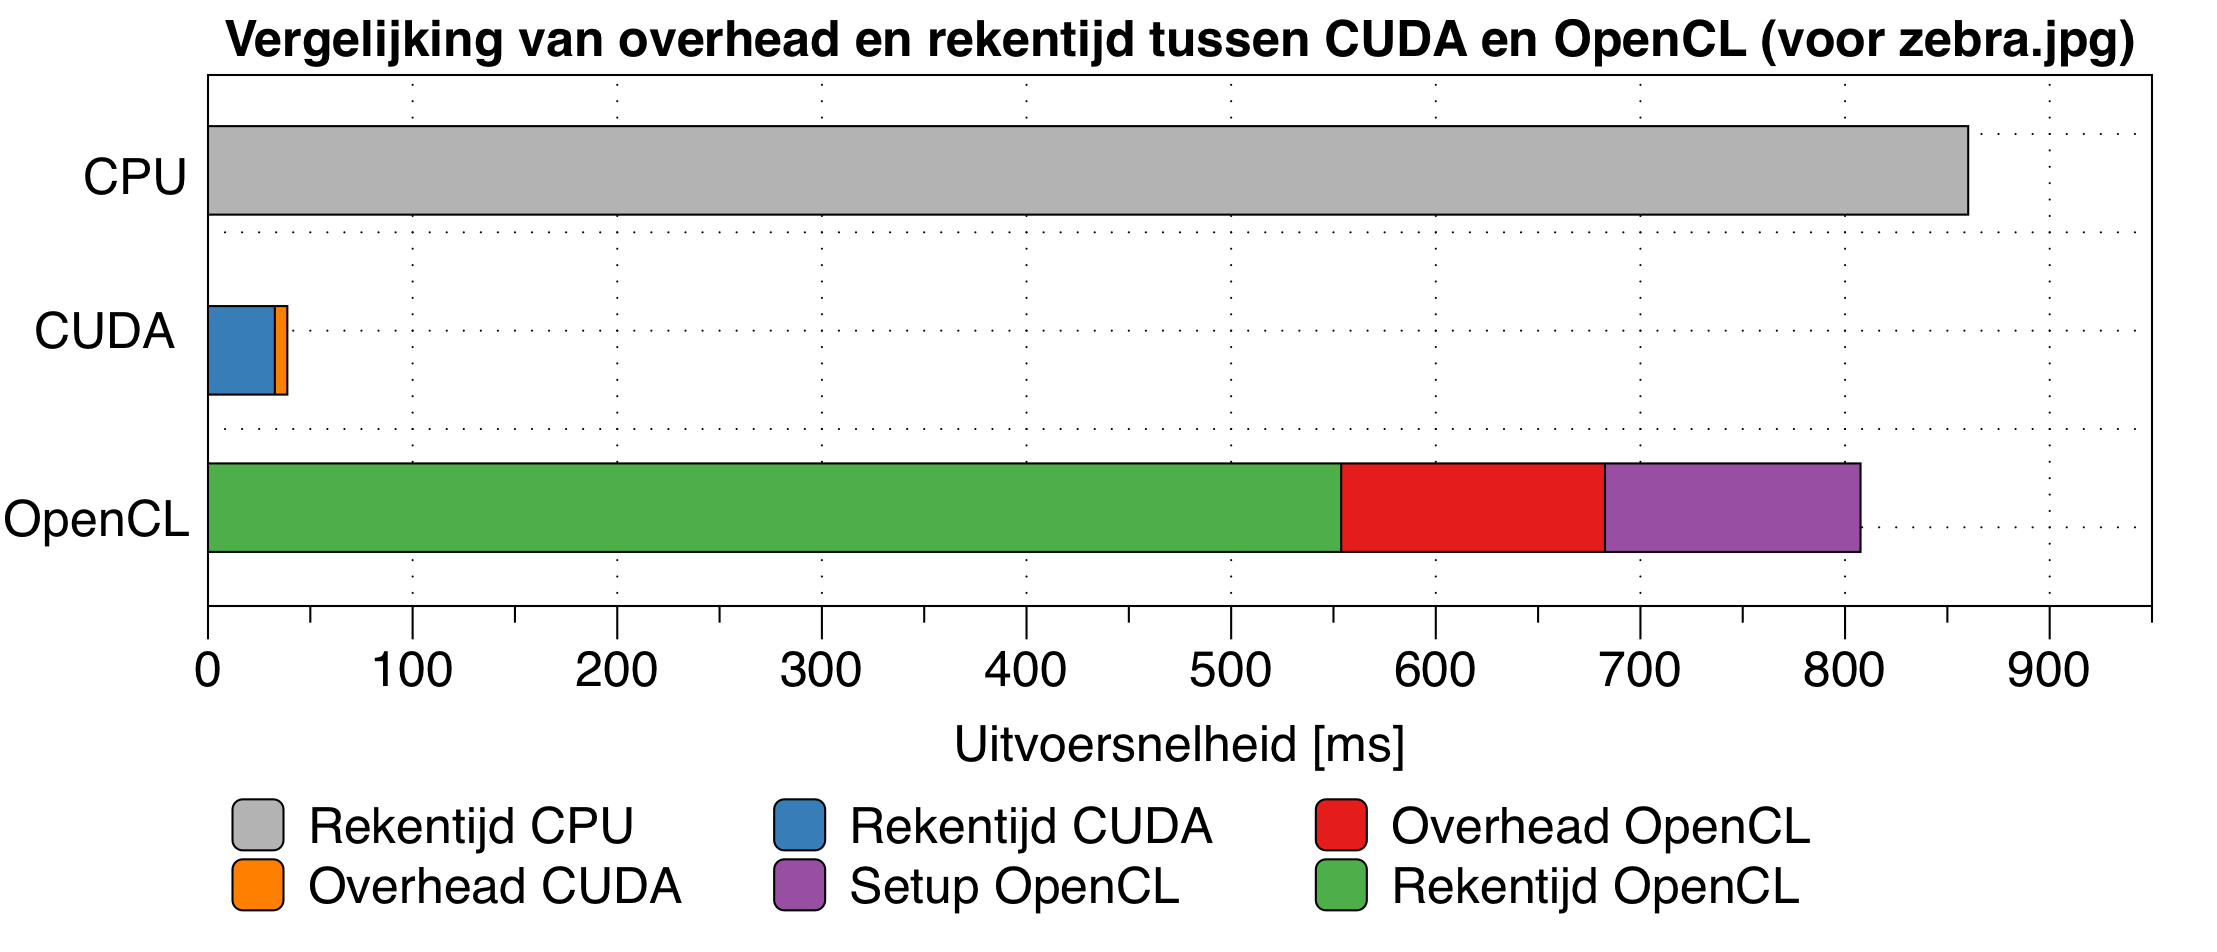
\includegraphics[width=0.48\textwidth]{data/opencl-vs-cuda-overhead.png}
    \caption{Overhead van Gaussiaans vervagen \\in OpenCL, CUDA en op de CPU.}\label{fig:vs-overhead}
\end{figure}

\section{Besluit}
Dit verslag werd geschreven als een extra opdracht voor het labo `Geavanceerde computerarchitectuur'. Een pipeline om afbeeldingen te bewerken met behulp van \textit{masks} werd opgezet en ge\"evalueerd.

Op basis van een van de geïmplementeerde operaties zijn drie aspecten van OpenCL geanalyseerd. Ten eerste is de invloed van de \emph{work size} voor een kernel bekeken, mocht deze op een GPU (in dit geval van AMD) draaien. Hieruit is geconcludeerd dat 64 of een veelvoud hiervan voor GPU's van AMD de beste optie was. OpenCL biedt ook de mogelijkheid om dit automatisch in te stellen, wat dan ook gedaan is voor de tweede evaluatie.

Als tweede aspect zijn verschillende devices met elkaar vergeleken voor het beoogde doel: foto's ontwikkelen. Hiervoor heeft een GPU duidelijk een snelheidsvoordeel ten opzichte van de CPU. Maar ook voor een CPU biedt OpenCL een voordeel, aangezien alle beschikbare cores ook gebruikt kunnen worden met dezelfde kernel. Niet alle apparaten werken echter even vlot, zo beïndigt de interne GPU van Intel regelmatig de OpenCL-kernels. 

Als derde aspect is OpenCL vergeleken met CUDA. Hierbij bleek CUDA ongeveer 20x sneller te zijn voor alle metingen. Aangezien dit op dezelfde GPU is uitgevoerd, zou dit significant verschil te wijten kunnen zijn aan beperkte ondersteuning voor OpenCL van NVIDEA. OpenCL is tenslotte op veel vlakken een concurrerend systeem, met een open karakter. 

\begin{figure*}
    \centering
    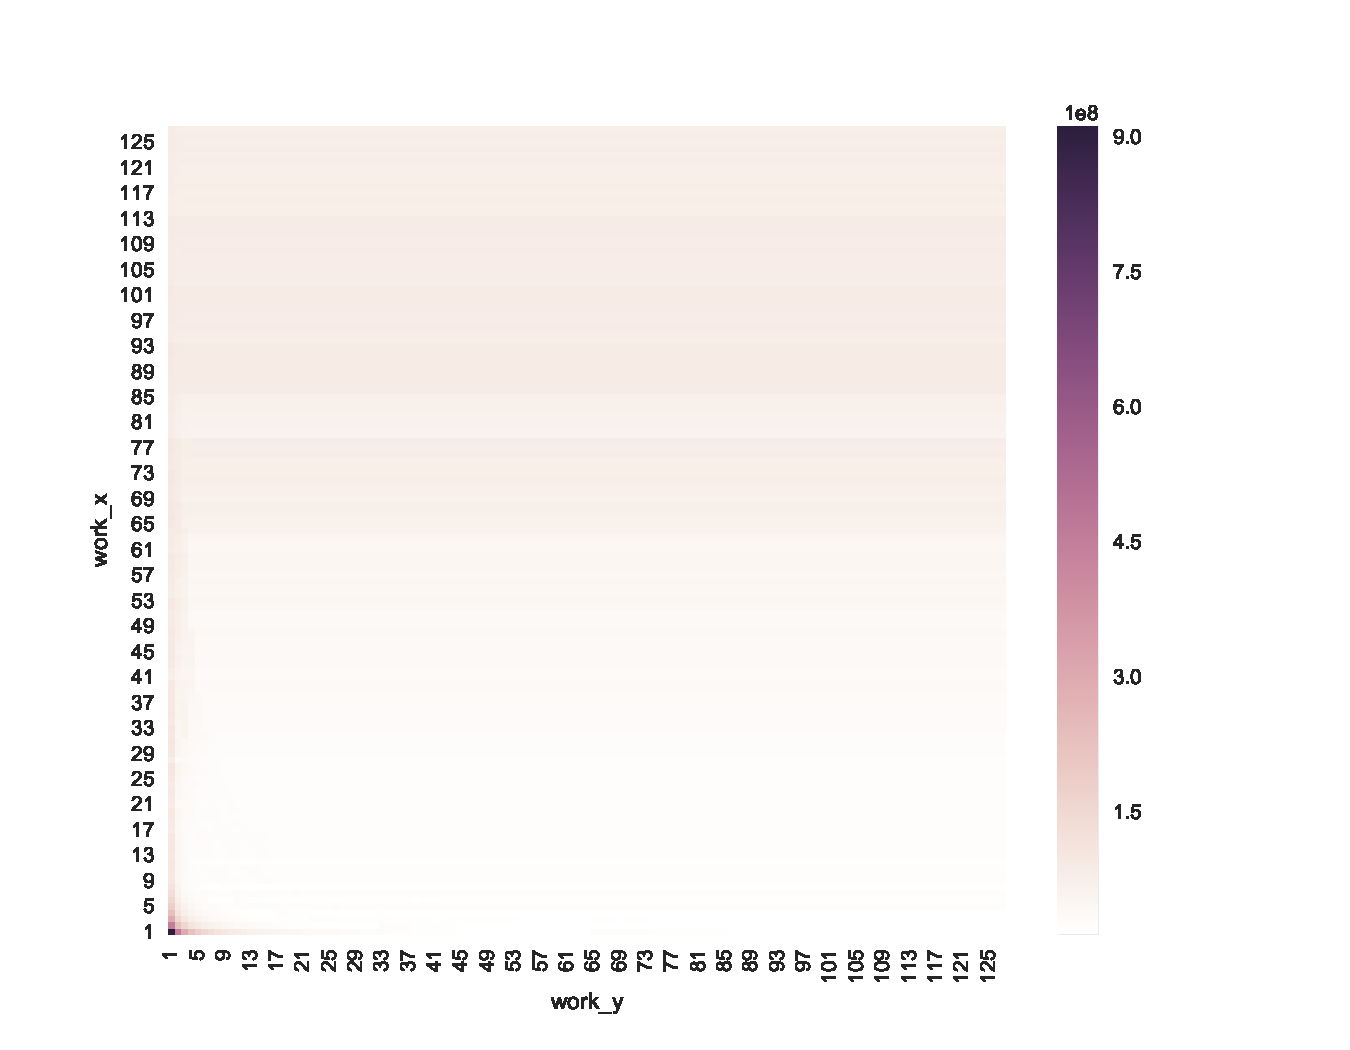
\includegraphics[width=1.1\textwidth]{data/output_powers.pdf}
    \caption{Invloed van een tweedimensionale \emph{work size} op uitvoertijd (in ns).}\label{fig:output-all}
\end{figure*}

\onecolumn

\appendix
\section{kernel.cl}
\inputminted[tabsize = 4, obeytabs, breaklines]{c}{../../code/zebra/test.cl}

\newpage

% The appendix command is issued once, prior to all appendices, if any.
%\appendix
\end{document}

